\documentclass[a4paper,11pt]{paper}

\usepackage[pdftex]{graphicx}
\usepackage{color}

\title{ColouredTree: a BEAST 2 framework for describing
phylogenies within structured populations}

\author{Tim Vaughan}

\newcommand{\class}[1]{\textsf{#1}}
\newcommand{\project}[1]{\textsf{#1}}
\newcommand{\inp}[1]{\textsf{\color{blue}#1}}
\newcommand{\code}[1]{\texttt{#1}}

\begin{document}

\maketitle

\section{Introduction}

BEAST 2 (hereafter simply referred to as BEAST) currently provides no
native way of handling true coloured trees---i.e., phylogenetic trees
corresponding to lineages evolving within some kind of structured
population. While it is true that BEAST has a useful facility for
recording arbitrary metadata in the form of ``traits'' on tree nodes,
information cannot be modified by BEAST Operators.  Without this
capability, geographic model parameters such as migration rates are
beyond the scope of the inference apparatus.

This document describes some first steps towards addressing these
shortcommings.

\section{State of the project}
Before going into the details of the plugin itself, let's consider the
current state of the development. So far, we have in place
\begin{itemize}
	\item a plugin for representing coloured trees,
	\item a plugin for initialising coloured trees from the structured
		coalescent, and
	\item a means of visualising coloured trees using Alexei's
		\project{beast-graphics} project.
\end{itemize}
These are the items which are described in the present document.

On the to-do list are the following (more challenging) items:
\begin{itemize}
	\item proposal operators for modifying colour assignments,
	\item calculation nodes for determining likelihoods of particular
		colour assignments.
\end{itemize}
Note that specific likelihoods and proposal operators depend on the
underlying structural model the colours represent, so we firstly need
to implement a general framework for such operators, then implement
some specific common cases (such as those relating to models of
migration between demes).

\section{Implementation of Coloured Trees (ColouredTree plugin)}

The first and most important point about the way in which coloured
trees are implemented is that the main class, \class{ColouredTree},
extends \class{Plugin}---it does not extend \class{Tree}.  As such,
\class{ColouredTree}s are not \class{StateNodes}, and cannot be used
directly in an MCMC calculation.  Instead, \class{ColouredTree} takes
a \class{Tree} as the input \inp{tree}, along with three parameter arrays which
are used to record the colouring information. The three parameter
array inputs are:
\begin{description}
	\item[\inp{changeCounts}]: an \class{IntegerParameter} array which
		is used to record the number of colour changes along each
		branch,
	\item[\inp{changeColours}]: another \class{IntegerParameter}
		array used to record the actual colours each change results
		in, and
	\item[\inp{changeTimes}]: a \class{RealParameter} array used to
		record the times (heights) at which the colour change events
		occur.
\end{description}

The counts in the \inp{changeCounts} array are indexed by the node
numbers (obtained via \code{node.getNodeNr()}) of the nodes on the
leaf-side of each branch.  The length of this array is equal to the
number of branches in \inp{tree}.

The colours in \inp{changeColours} and times in \inp{changeTimes} are
stored as flattened matrices, with the row identified by the leaf-side
node number and the column given by a number between 0 and one less
than the change count for the branch specifying that particular
change. Note that as the total length of \class{Parameter} arrays
cannot change once they are initialised, the dimension of
\inp{changeTimes} and \inp{changeColours} must be fixed.  It is thus
necessary to set an upper bound on the total number of changes which
can occur along any branch, and this is specified via the input
\inp{maxBranchColours}.

Clearly the way in which the colour information is stored in these
\class{Parameters} fairly cumbersome. This is a necessary evil
as, unlike \class{ColouredTree}, \class{Parameter}s \emph{do} extend
\class{StateNode} and may thus form part of the state in an MCMC
calculation. However, they should not be accessed directly either by
\class{Operator}s or methods involved in the creation of
\class{ColouredTree} objects. Instead, \class{ColouredTree} exposes a
set of helper methods which allow the colouring information to be
handled in a more intuitive way.

\subsection{Other ColouredTree inputs}

Before moving on to describing these helper methods, however, we will
briefly describe the other inputs to \class{ColouredTree}. 

\subsection{ColouredTree methods}

\begin{figure}
	\centering
	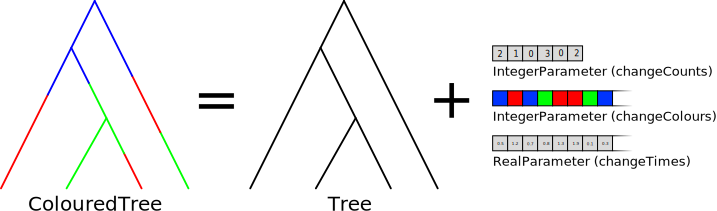
\includegraphics[width=\textwidth]{treeComposition.pdf}
	\caption{Composition of the \class{ColouredTree} plugin.}
\end{figure}

\section{Generating Coloured Trees (StructuredCoalescentColouredTree plugin)}



\subsection{StructuredCoalescentColouredTree inputs}
\subsection{StructuredCoalescentColouredTree methods}

\begin{figure}
	\centering
	\includegraphics[width=0.5\textwidth]{structuredCoalescentFig.pdf}
	\caption{Coloured tree generated using
		\class{StructuredCoalescentColouredTree} and visualised using
	\project{beast-graphics}.}
\end{figure}

\section{Interfacing with {\textsf beast-graphics} (FlatColouredTree plugin)}

\subsection{FlatColouredTree inputs}
\subsection{FlatColouredTree methods}

\end{document}
